\documentclass[xcolor={table,dvipsnames}]{beamer}
\usepackage[utf8]{inputenc}
\usetheme{CambridgeUS}
\definecolor{darkred}{rgb}{0.2,0.2,0.7}
\setbeamercolor{title}{bg=gray!15!white}
\setbeamercolor{block title}{bg=gray!30!white}
\setbeamercolor{alerted text}{fg=orange!90!brown}
\renewcommand{\emph}[1]{\textit{\color{orange!90!brown}#1}}
\newcommand{\faint}{\color{black!10!gray}}
\beamertemplatenavigationsymbolsempty
\graphicspath{{figures/}}

\usepackage{listings}
\lstdefinestyle{Bash}{language=Bash,commentstyle=\color{gray}}
\lstset{basicstyle=\ttfamily\color{darkred},columns=fullflexible}
\lstset{keepspaces=true,style=Bash,gobble=8}
\newcommand{\bashcmd}[2][-0.6\baselineskip]{%
  \lstinputlisting{#2}%
  \vspace{#1}%
}
\newcommand{\bashout}[2][-0.1\baselineskip]{%
  \lstinputlisting[basicstyle=\ttfamily\color{black!80}]{#2}%
  \vspace{#1}%
}

\author{Björn Bastian}
\title[Citation tools]{Command line tools for bibtex citations}

\begin{document}

\begin{frame}[plain]
  \titlepage
\end{frame}

\begin{frame}{Contents}
  \tableofcontents
\end{frame}

\section{Typical use}

\subsection{Getting new literature}
\begin{frame}{Getting new literature}
  \begin{minipage}[t]{.6\textwidth}
    \vspace{-0.6\baselineskip}
    \uncover<1->{\bashcmd{cmdline/new/d1-1-in.txt}}%
    \uncover<1->{\bashout{cmdline/new/d1-1-out.txt}}%
    \uncover<3->{\bashcmd{cmdline/new/d1-2-in.txt}}%
    \uncover<3->{\bashout{cmdline/new/d1-2-out.txt}}%
    \uncover<4->{\bashcmd{cmdline/new/d1-3-in.txt}}%
    \uncover<4->{\bashout{cmdline/new/d1-3-out.txt}}%
  \end{minipage}%
  \hfill%
  \begin{minipage}[t]{.34\textwidth}
    \hbox{\;}
    \only<1>{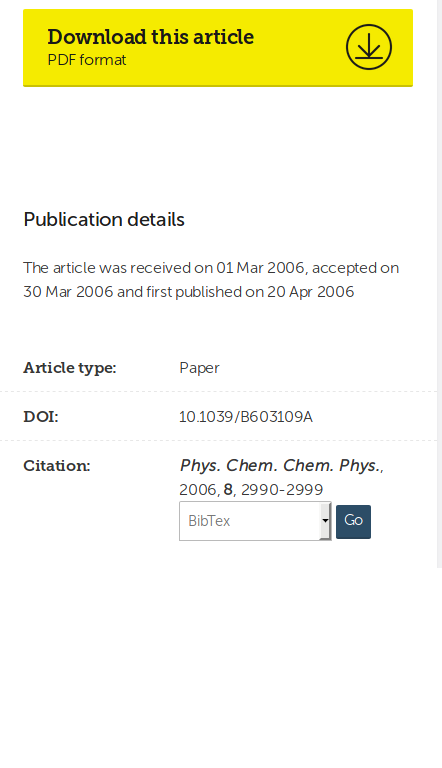
\includegraphics[width=\textwidth]{new/d1-0.png}}%
    \only<2>{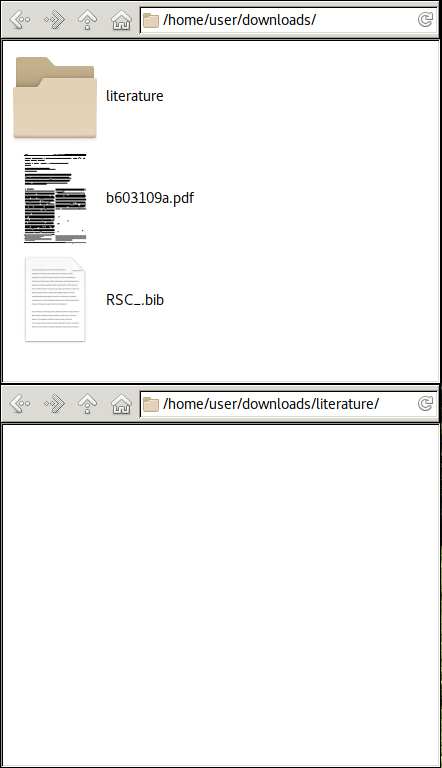
\includegraphics[width=\textwidth]{new/d1-1.png}}%
    \only<3->{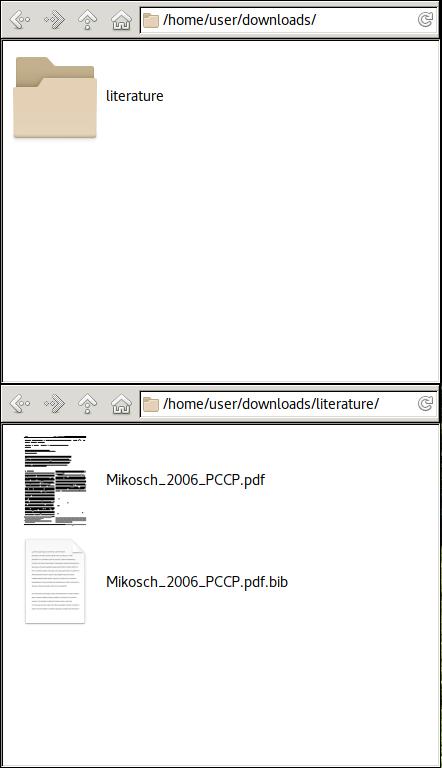
\includegraphics[width=\textwidth]{new/d1-2.png}}%
  \end{minipage}%
\end{frame}

\subsection{Multi record files}
\begin{frame}{Multi record files}
  \bashcmd[0pt]{cmdline/all/d2-1-in.txt}
  \begin{center}
    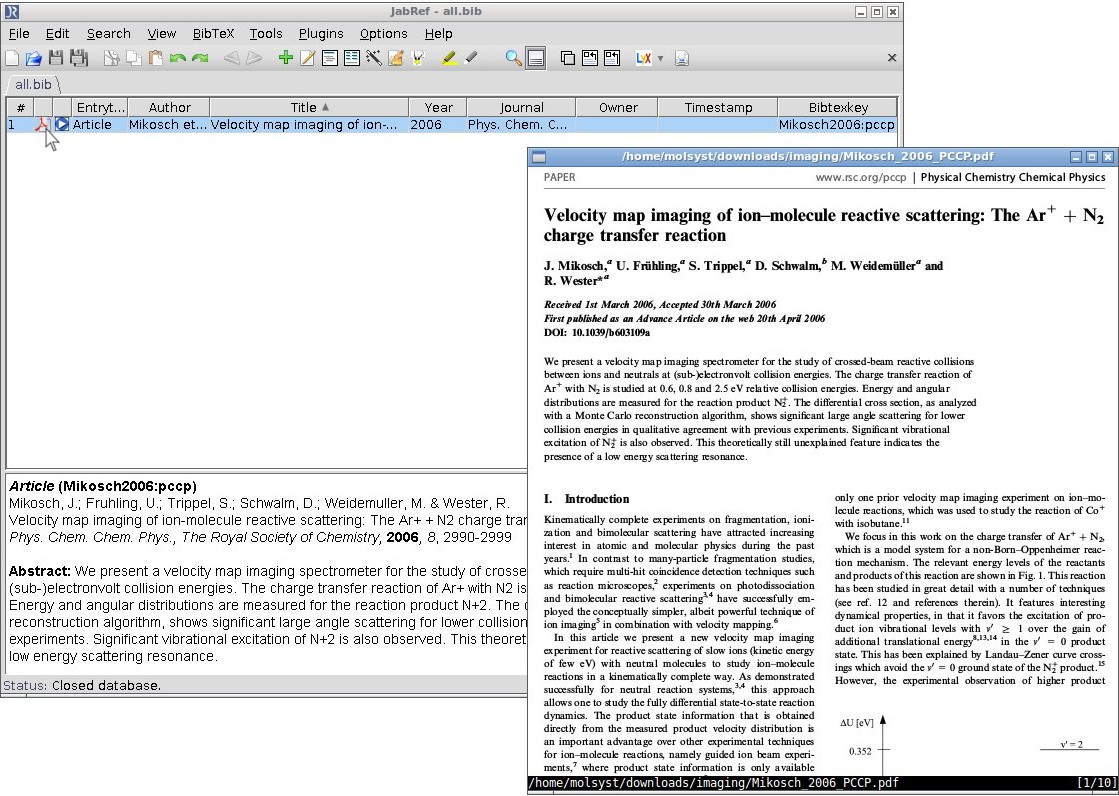
\includegraphics[height=.7\textheight,trim=0 120 0 0,clip]{jabref.jpg}
  \end{center}
\end{frame}

\subsection{Sort in directories}
\begin{frame}{Sort in directories}
  \begin{minipage}[t]{.6\textwidth}
    \vspace{-0.6\baselineskip}
    \uncover<1->{\bashcmd{cmdline/dirs/d3-1-in.txt}}%
    \uncover<1->{\bashout{cmdline/dirs/d3-1-out.txt}}%
    \uncover<2->{\bashcmd{cmdline/dirs/d3-2-in.txt}}%
    \alt<1-3>{%
      \uncover<2-3>{\bashout{cmdline/dirs/d3-2-out.txt}}%
    }{%
      \uncover<4->{\bashout[-0.6\baselineskip]{cmdline/dirs/d3-2-out-alt.txt}}%
      \uncover<4->{\bashcmd{cmdline/dirs/d3-3-in.txt}}%
      \uncover<4->{\bashout{cmdline/dirs/d3-3-out.txt}}%
    }%
    \uncover<5->{\bashcmd{cmdline/dirs/d3-4-in.txt}}%
  \end{minipage}%
  \hfill%
  \begin{minipage}[t]{.34\textwidth}
    \hbox{\;}
    \only<1>{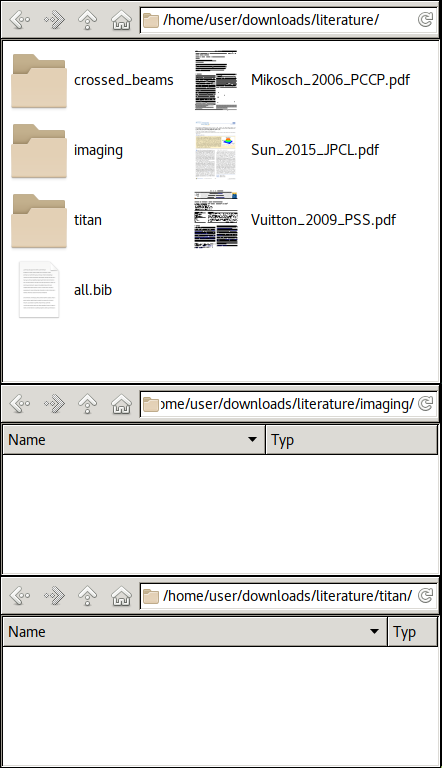
\includegraphics[width=\textwidth]{dirs/d3-1.png}}%
    \only<2>{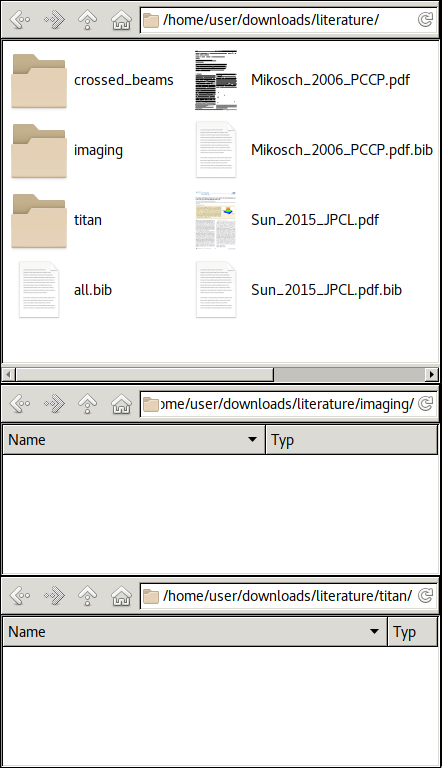
\includegraphics[width=\textwidth]{dirs/d3-2.png}}%
    \only<3-4>{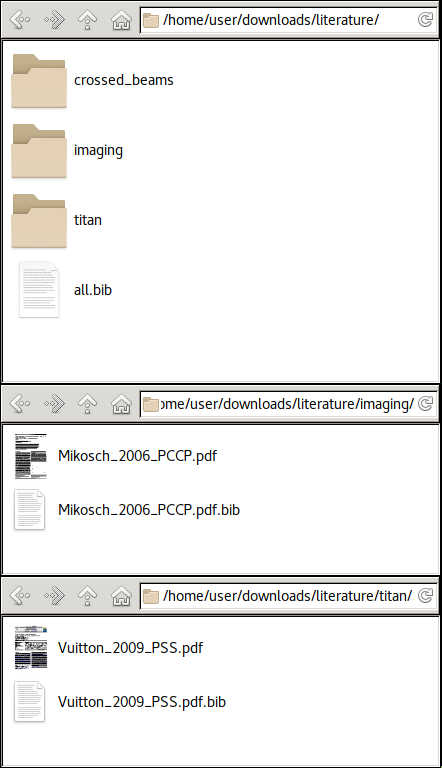
\includegraphics[width=\textwidth]{dirs/d3-3.png}}%
    \only<5>{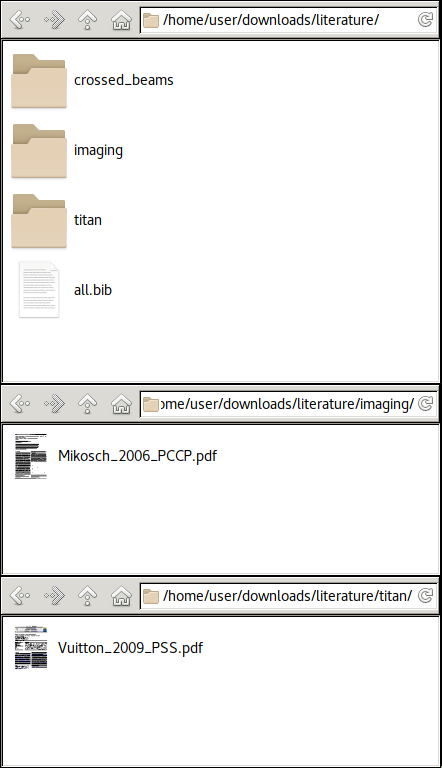
\includegraphics[width=\textwidth]{dirs/d3-4.png}}%
  \end{minipage}%
\end{frame}

\section{All command line tools}

\subsection{Overview}
\begin{frame}{All command line tools}
  \vspace{-3pt}
  \begin{itemize}
    \itemsep-10pt

    \item Formatting, filename and citation key
      \begin{tabbing}
        \texttt{bib-longest, newbib} \= Description \kill
        \texttt{bib-format} \> Format bibtex file \\
        \texttt{bib-keyinsert} \> Create citation key \\
        \texttt{bib-name} \> Rename bibtex and pdf file \\
        \alert<1>{\texttt{newbibpdf}}, \texttt{newbib} \> Combine the 3 above tasks \\
      \end{tabbing}

    \item Multi record files
	\hfill\alert{already seen}\quad\hbox{\,}
      \begin{tabbing}
        \texttt{bib-longest, newbib} \= Description \kill
        \alert{\texttt{bib-pdfinsert}} \> Link to pdf file for JabRef \\
        \alert{\texttt{bib-unite}} \> Unite and sort bibtex files \\
        \alert{\texttt{bib-separate}} \> Split bibtex files by key of pdf path \\
        \texttt{bib-extract} \> Extract bibtex entries by key matching \\
        \texttt{bib-order} \> Sort a multi record file by key \\
        \texttt{bib-merge} \> Merge bibtex entries to one target file \\
      \end{tabbing}

    \item Some more tools
      \begin{tabbing}
        \texttt{bib-longest, newbib} \= Description \kill
        \texttt{bib-jabbr} \> (Un)abbreviate journal names \\
        \texttt{bib-txt} \> Plain text formatted citations \\
      \end{tabbing}

    \end{itemize}
\end{frame}

\subsection{Some more tools}
\begin{frame}[fragile]{Some more tools}
  \begin{itemize}

    \item \emph{Abbreviate} or unabbreviate
      (option {\faint\verb!-u!}) \emph{journal names}
      \bashcmd{cmdline/jabbr/jabbr-1-in.txt}
      \bashout{cmdline/jabbr/jabbr-1-out.txt}

    \item Extract bibtex entries by \emph{matching patterns} against the citation key
      \begin{lstlisting}
        $ bib-extract all.bib Mikosch    # Match author
        $ bib-extract all.bib 2006:pccp  # Match year & journal
        $ bib-extract all.bib 2006 pccp  # Match either
      \end{lstlisting}

    \item Get \emph{plain text citations} from bibtex files
      \begin{lstlisting}
        $ bib-txt article.bib # Use option -f to change format
        $ bib-extract all.bib Mikosch | bib-txt - # From stdin
      \end{lstlisting}
      {\faint\footnotesize Mikosch, J., Frühling, U., Trippel, S., Schwalm, D.,
	Weidemüller, M., Wester, R., Phys. Chem. Chem. Phys., 8, 2990 (2006) }

  \end{itemize}
\end{frame}

\subsection{Adding new files}
\begin{frame}[fragile]{Adding new pdf+bibtex files (\texttt{newbibpdf/newbib})}
  \begin{itemize}

    \item For bibfiles without pdf, call \texttt{\color{darkred}newbib bibfiles} instead

    \item \emph{Format, rename} and \emph{create cite key} for a bib and pdf file\\
      \begin{lstlisting}
        $ newbibpdf article.pdf article.bib
        $ newbibpdf article.pdf
	$ newbibpdf # .bib/.pdf files unique in directory
	$ newbibpdf -l # choose newest files in directory
      \end{lstlisting}

    \item The same with a \emph{target directory} other than \verb!new_lit!
      \begin{lstlisting}
        $ newbibpdf imaging article.pdf
      \end{lstlisting}

    \item[$\Rightarrow$] {\faint\verb!b603109a.pdf!} and {\faint\verb!RSC_.bib!}
      were \emph{moved} to {\faint\verb!imaging!} directory as
      {\faint\verb!Mikosch_2006_PCCP.pdf!} and
      {\faint\verb!Mikosch_2006_PCCP.pdf.bib!}

    \item[$\Rightarrow$] The \emph{citation key} {\faint\verb!Mikosch2006:pccp!} was inserted

    \item[$\Rightarrow$] The bib file was \emph{formatted}
      (option {\faint\verb!-u!} skips content changes)

  \end{itemize}
\end{frame}

\begin{frame}[fragile]{Step by step (what \texttt{newbibpdf/newbib} do)}
  \begin{tabbing}
    Note: \=use option {\faint\verb!-n!} to only view changes
                   and {\faint\verb!-h!} to see all options; \\
	  \>the options {\faint\verb!-n!}, {\faint\verb!-u!} and
	  {\faint\verb!-f!} are also supported by \texttt{newbibpdf}
  \end{tabbing}

  \begin{itemize}

    \item \emph{Format} bibtex file
      \begin{lstlisting}
        $ bib-format -u article.bib  # Format structure only
        $ bib-format -n article.bib  # View content changes
        $ bib-format article.bib
      \end{lstlisting}

    \item Use journal name \emph{abbreviation}
      \begin{lstlisting}
	$ bib-jabbr article.bib  # Option -f for full name
      \end{lstlisting}

    \item Create and update \emph{citation key}
      \begin{lstlisting}
        $ bib-keyinsert article.bib
      \end{lstlisting}
      \vspace{-0.5\baselineskip}
      \hfill{\faint\verb!@Article{Mikosch2006:pccp!}

    \item Show new filenames and \emph{rename} files
      \begin{lstlisting}
        $ bib-name article.bib
      \end{lstlisting}

  \end{itemize}
\end{frame}

\begin{frame}[fragile]{Formatting (what \texttt{bib-format} does)}
  \begin{itemize}

    \item \emph{Journal names} without "The" prefix and whitespace\\
      $\rightarrow$ JabRef or \texttt{bib-jabbr} can abbreviate them

      {\faint\verb!   Journal = {Journal of Chemical Physics},!}
      {\faint\verb!   Journal = {J. Chem. Phys.},!}

    \item Single spacing for \emph{abbreviated forenames}\\
      $\rightarrow$ second forenames do not disappear in {\small PDF}

      {\faint\verb!   Author  = {... and Gianturco, F. A.},!}

    \item Remove \emph{url} and html part from \emph{doi} if defined\\
      $\rightarrow$ no additional links in the references

      {\faint\verb!   Doi     = {10.1039/B603109A},!}

    \item \emph{Unified formatting} and indentation in  JabRef style, e.\,g.
      \begin{itemize}
        \item use curly brackets (often double quotes are used)
        \item homogeneous indentation, title case keys
      \end{itemize}

    \item Replace utf8 characters, escape ampersands, \ldots

  \end{itemize}
\end{frame}

\subsection{Multi record files}
\begin{frame}[fragile]{Multi record files}
  \begin{itemize}

    \item Sorted \emph{concatenation} of selected bib files
      \begin{lstlisting}
	$ bib-pdfinsert */*.bib        # File links for JabRef
        $ bib-unite */*.bib > all.bib
      \end{lstlisting}

    \item Same with \emph{recursive search} of all bib files in subdirectories
      \begin{lstlisting}
        $ find */ -name "*.bib" -exec bib-pdfinsert {} \;
        $ find */ -name "*.bib" | xargs bib-unite > all.bib
        $ find */ -name "*.bib" -delete  # Be careful
      \end{lstlisting}

    % \item Only consider bib files with a reference to the pdf file
    %   \begin{lstlisting}
    %     $ find . */ -name "*.bib" \
    %         -exec grep -l "File *=" {} \; \
    %         | xargs bib-unite > all.bib
    %   \end{lstlisting}

    \item \emph{Split} multi record file: entries are written
      to single files according\\
      to the \verb!File! links (if available) or the citation key
      \begin{lstlisting}
        $ bib-separate all.bib
        $ bib-separate all.bib -k  # Only use keys (not File)
      \end{lstlisting}

    \item \emph{Sort} multi record file by citation key
      \begin{lstlisting}
        $ bib-order all.bib      # Option -c checks if sorted
      \end{lstlisting}

  \end{itemize}
\end{frame}

\subsection{Merging bibtex files}
\begin{frame}[fragile]{Merging bibtex files}
  \begin{itemize}

    \item \emph{Merge} several files into one target file
      \begin{lstlisting}
	$ bib-merge target.bib *.bib
      \end{lstlisting}

      \begin{itemize}
	\item Preprocesses files to be merged, queries user before changes.
	\item Keys that already exist in the target file ared skipped.
	\item Check manually for differing entries with identical keys.
      \end{itemize}

    \item Print \emph{duplicate} keys
      \begin{lstlisting}
	$ bib-keyinsert -d *.bib
      \end{lstlisting}

    \item \emph{Unite} several files
      {\color{gray}(sort by key and year, option -r for newest first)}
      \begin{lstlisting}
	$ bib-unite -d *.bib > united.bib
      \end{lstlisting}

      \begin{itemize}
	\item Unites all entries except for exact duplicates that are dropped.
	\item Afterwards, resolve remaining duplicate keys manually.
      \end{itemize}

  \end{itemize}
\end{frame}

\subsection{Ambiguous keys}
\begin{frame}{Ambiguous keys (option 1 using \texttt{bib-keyinsert})}
  \begin{itemize}[<+->]
    \item The issue of \emph{non unique} citation keys
      \bashcmd{cmdline/key/uniq-1-in.txt}
      \bashout{cmdline/key/uniq-1-out.txt}

    \item Choose suffixes a and b as \emph{filename:x}
      \bashcmd{cmdline/key/uniq-2-in.txt}
      \bashout{cmdline/key/uniq-2-out.txt}

    \item Citation key suffixes are used for filenames
      \bashcmd{cmdline/key/uniq-3-in.txt}
      \bashout{cmdline/key/uniq-3-out.txt}
  \end{itemize}
\end{frame}

\begin{frame}{Ambiguous keys (option 2 using \texttt{bib-name})}
  \begin{itemize}[<+->]
    \item The issue of \emph{non unique} citation keys
      \bashcmd{cmdline/name/uniq-1-in.txt}
      \bashout{cmdline/name/uniq-1-out.txt}

    \item Choose suffixes a and b as \emph{filename:x}
      \bashcmd{cmdline/name/uniq-2-in.txt}
      \bashout{cmdline/name/uniq-2-out.txt}

    \item Filename year suffixes are used for citation keys
      \bashcmd{cmdline/name/uniq-3-in.txt}
      \bashout{cmdline/name/uniq-3-out.txt}
  \end{itemize}
\end{frame}

\end{document}
